\documentclass[a4paper,12pt]{article}

\usepackage{latexsym}
\usepackage[utf8]{inputenc}
\usepackage{graphicx}
\author{Krzysztof~Palka and Dominik~Odrowski}

\title{\textsc{Exercise} 421 \\ Examination of light polarization by reflection phenomena} 
\begin{document}
\maketitle

\begin{abstract}
    This report present the measurement of Brewster's angle for a given material. It shows relation of level of ray polarization depending on incident angle of unpolarized light.    
\end{abstract}

\section{Introduction}
The aim of this exercise was determining of Brewster's angle for given material and, depending on obtained results, calculation of index of reflection. 


\section{Theory and measurement}
The light polarized randomly (or unpolarized) is characterized by electric filed at any given point perpendicular to the direction of travel of the waves but changes directions randomly. We can treat unpolarized light as combination of two perpendicular components (polarization S and P) which oscillate perpendicular to component of the electric field (Fig. \ref{fig:sp}\footnote{\cite{HRW}, p. 901}). 

\begin{figure}[h]
\begin{center}
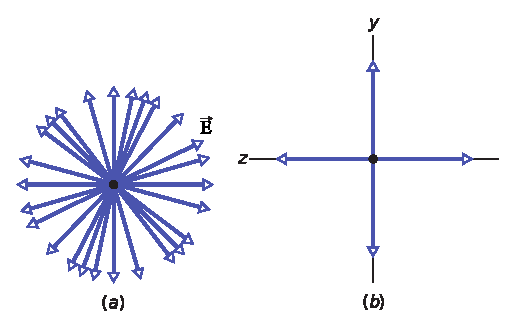
\includegraphics[width=0.65\textwidth]{simplified_polarization}
\caption{polarization (a) could be simplified as (b)}
\label{fig:sp}
\end{center}
\end{figure}

\begin{thebibliography}{2}
    \bibitem[HRW]{HRW}Fundamentals of physics (2011) [ebook]. David Halliday, Robert Resnick, Jearl Walker. 9th ed. ISBN 978-0-470-46908-8
\end{thebibliography}
\end{document}

